\addcontentsline{toc}{chapter}{Appendices}

% The \appendix command resets the chapter counter, and changes the chapter numbering scheme to capital letters.
%\chapter{Appendices}
\appendix
\chapter{Datasets used}
\label{appendixlabel1}

This appendix described the different datasets used in analyses performed in this thesis. It includes datasets of both modern and ancient genomes 

\section{Antonio et al 2019}

Samples from Antonio et al (2019)\cite{antonio2019ancient}. Looking at the population genomics of ancient Rome. 

This dataset consists of 134 shotgun-sequenced individuals from 12,000 years ago to the present day. Coverage ranges from 0.4x - 4x (median 1.05x). 

Aligned reads in .bam format were downloaded from the ENA under accession number PRJEB32566.

\section{Margaryan et al 2020}

Samples from Margaryan et al 2020 \cite{margaryan2020population}, looking at the population genomics of Vikings.  

This dataset consists of 442 shotgun-sequenced individuals from the Bronze Age to Medieval and Early Modern ages. Mean coverage of ~1x. X individuals did not have enough data to estimate recalibration parameters and were excluded from the rest of the analysis.

Aligned reads in .bam format were downloaded from the ENA under accression number PRJEB37976. 

\section{Rivollat et al 2020}

Samples from Rivollat et al (2020)\cite{rivollat2020france}. Looking at the population genomics of France and Germany. 

This dataset consists of 101 captured individuals from 7000–3000 BCE. years ago to the present day. 

Aligned reads in .bam format were downloaded from the ENA under accession number PRJEB36208.


\section{Brunel et al 2018}

Samples from Brunel et al (2018)\cite{Brunel12791}. Looking at the population genomics of France. 

This dataset consists of 52 shotgun sequenced individuals from Mesolithic to the Iron Age. 

Aligned reads in .bam format were downloaded from the ENA under accession number PRJEB36208.

\section{Allentoft et al 2015}

Samples from Allentoft et al 2015 \cite{Allentoft2015}. Looking at the population genomics Bronze Age Eurasia. 

This dataset consists of 20 shotgun sequenced individuals. 

Aligned reads in .bam format were downloaded from the ENA under accession number PRJEB9021.

\section{Broushaki et al 2016}

Samples from Broushaki et al 2016 \cite{Broushaki2016b}. Looking at the population genomics Bronze Age Eurasia. 

This dataset consists of 1 shotgun sequenced individual.

Aligned reads in .bam format were downloaded from the ENA under accession number xxxx.

\section{Cassidy et al 2016}

Samples from Cassidy et al 2016 \cite{Cassidy368}. Looking at the population genomics of the Neolithic and Bronze Age migrations to Ireland. 

This dataset consists of 4 shotgun sequenced individuals.

Aligned reads in .bam format were downloaded from the ENA under accession number PRJEB11995.

\section{de Barros Damgaard et al 2018a}

The first horse herders and the impact of early Bronze Age steppe expansions into Asia.

Samples from de Barros Damgaard et al 2018a \cite{deBarrosDamgaardeaar7711}.

This dataset consists of 34 shotgun sequenced individuals.

Aligned reads in .bam format were downloaded from the ENA under accession number PRJEB26349.

\section{de Barros Damgaard et al 2018b}

137 ancient human genomes from across the Eurasian steppes

Samples from de Barros Damgaard et al 2018b \cite{de2018137}.

This dataset consists of 58 shotgun sequenced individuals.

Aligned reads in .bam format were downloaded from the ENA under accession number PRJEB20658.

\section{Gamba et al 2014}

Genome flux and stasis in a five millennium transect of European prehistory

Samples from  Gamba et al 2014 \cite{Gamba2014}.

This dataset consists of 10 shotgun sequenced individuals.

Aligned reads in .bam format were downloaded from the Sequence Read Archive (SRA) under the accession code SRP039766.

\section{Gunther et al 2015}

Genomic diversity and admixture differs for Stone-Age Scandinavian foragers and farmers

Samples from Gunther et al 2015 \cite{gunther2015ancient}.

This dataset consists of 2 shotgun sequenced individuals.

Aligned reads in .bam format were downloaded from the ENA under accession number PRJEB9783.

\section{Hofmanová et al 2016}

Early farmers from across Europe directly descended from Neolithic Aegeans

Samples from  Hofmanová et al 2016 \cite{Hofmanova2016}.

This dataset consists of 5 shotgun sequenced individuals.

Aligned reads in .bam format were downloaded from the ENA under accession number PRJEB11848.

\section{Jones et al 2015}

Upper Palaeolithic genomes reveal deep roots of modern Eurasians

Samples from  Jones et al 2015 \cite{Jones2015}.

This dataset consists of 2 shotgun sequenced individuals.

Aligned reads in .bam format were downloaded from the ENA under accession number PRJEB11364.

\section{Marchi et al 2020}

The mixed genetic origin of the first farmers of Europe

Samples from  Marchi et al 2020 \cite{marchi2020mixed}.

This dataset consists of 4 shotgun sequenced individuals.

Aligned reads in .bam format were downloaded from the ENA under accession number PRJEB11364.

\section{Olalde et al 2014}

\textbf{Derived immune and ancestral pigmentation alleles in a 7,000-year-old Mesolithic European}

Samples from  Olalde et al 2014 \cite{olalde2014derived}.

This dataset consists of 1 shotgun sequenced individual.

Aligned reads in .bam format were downloaded from the ENA under accession number PRJNA230689.

\section{Sánchez-Quinto et al 2019}

\textbf{Megalithic tombs in western and northern Neolithic Europe were linked to a kindred society}

Samples from  Sánchez-Quinto et al 2019 \cite{sanchez2019megalithic}.

This dataset consists of 7 shotgun sequenced individuals.

Aligned reads in .bam format were downloaded from the ENA accession number PRJNA230689.

\section{Seguin-Orlando et al 2014}

\textbf{Genomic structure in Europeans dating back at least 36,200 years}

Samples from  Seguin-Orlando et al 2014 \cite{Seguin-Orlando2014}.

This dataset consists of 1 shotgun sequenced individual.

Aligned reads in .bam format were downloaded from the ENA under accession number PRJNA230689.

\section{Ancient reference dataset} \label{AncientReferenceDataset}

This section describes the generation of the dataset of reference ancient individuals used in Chapters 2, 4 and 5. 

The following steps were used to generate the data:

\begin{enumerate}
\item Each \texttt{.bam} was processed with \texttt{PicardTools ValidateBam} \cite{Picard2018toolkit} task to ensure no files were corrupted or contained incorrect read group information.
\item Each \texttt{.bam} file was processed with atlas (version 1.0, commit f612f28) pipeline \cite{Link2017} (\url{https://bitbucket.org/wegmannlab/atlas/wiki/Home}). For .bam file, I estimated post-mortem damage (PMD) patterns using atlas \texttt{estimatePMD} task. Recalibration parameters were then estimated using atlas \texttt{recal} task. Finally, both the recalibration and PMD parameters were given to the \texttt{callNEW} task which produces genotype calls and genotype likelihood estimates for each downsampled and full coverage .bam. For this stage, I made calls at the 77,818,345 genome-wide positions present in the phase 3 thousand genomes project \cite{1000GenomesProjectConsortium2015}. This was done to reduce the risk of calling false-positive non-polymorphic sites. This resulted in a \texttt{.bcf} file for each ancient sample. 
\item All \texttt{.bcf} files were split into chromosomes and all samples from the same chromosome were merged. Imputation and phasing was performed with GLIMPSE (version 1.1.1). I followed the steps laid out in the GLIMPSE tutorial (\url{https://odelaneau.github.io/GLIMPSE/tutorial_b38.html}). First, I used \texttt{GLIMPSE\_chunk} to split up each reference chromosome into chunks, keeping both \texttt{--window-size} and \texttt{--buffer-size} to 2,000,000, their default settings. Across all chromosomes, this produced 936 chunks of an average 2.99Mb long. I used the b37 genetic map supplied by GLIMPSE for the \texttt{--map} argument. 

Each chunk was then imputed separately using \texttt{GLIMPSE\_phase} using the same 1000 genomes dataset as a reference. Default settings and the supplied b37 genetic map were used. This stage both imputes missing genotypes and generates a set of haplotype pairs which can be sampled from in a later step to produced phased haplotypes.

\texttt{GLIMPSE\_ligate} was then used to merge the imputed chunks back to form single chromosomes using the default settings and the supplied b37 genetic map. 

Haplotypes were then sampled using \texttt{GLIMPSE\_sample} to produce a .vcf with phased haplotypes for each individual, again using default settings and the supplied b37 genetic map. 

Consequently, the output of GLIMPSE is i) unphased genotype calls with posterior genotype likelihoods and ii) phased haplotypes.


\item Finally, the posterior genotype likelihoods and phased haplotypes were combined to generate ChromoPainterUncertainty output using a custom script (\url{https://github.com/sahwa/vcf_to_chromopainter}).



\end{enumerate}



\section{30x 1000 genomes dataset} \label{1000genomesdataset}

Samples from \cite{byrska2021high}.

This dataset consists of 3,202 modern individuals from 26 worldwide populations, sequenced to a targeted depth of 30x coverage. The downloaded dataset was aligned to the gr38 reference genome.

Samples were downloaded to the UCL Computer Science cluster by myself from the ftp mirror.

The following steps were taken to process the data before being used as an imputation reference. 

\begin{enumerate}
\item Filtered such that SNPs with only 2 alleles were retained
\item Performed a liftover to hg19 using LiftoverVcf from picard tools \cite{Picard2018toolkit}
\item Filter again for SNPs with only 2 alleles
\item Phase using shapeit4, using the `sequencing' parameter and setting --pbwt-depth 4.
\item Remove duplicated SNPs using bcftools norm \cite{li2009sequence} 
\item Use Beagle's conform-gt utility to ensure reference alleles were consistent with the previous 1000 genomes build. This was done because all previous datasets I have compiled were also conformed to the previous 1000 genomes build. 
\end{enumerate}

\section{Human Origins dataset} \label{HumanOriginsAppendix}

This dataset consists of 560,420 SNPS and 5998 individuals from 509 worldwide populations. It has a particularly large number of samples from West and East Africa; in particular, Cameroon, Ethiopia, Nigeria and Ghana. 

\subsection{Processing}

Only bi-allelic SNPs were retained. To ensure that all datasets, ancient and modern, can be merged together without the confounding effects of strand flips, I then used conform-gt (\url{https://faculty.washington.edu/browning/conform-gt.html}) to align all alleles to the same strand as the 1000 genomes reference, keeping all parameters as default. Any genotypes which had a genotype likelihood of below 0.990 were set as missing.

Data was phased use \texttt{shapeit4} \cite{delaneau2018integrative}, setting \texttt{--pbwt 8} and keeping all other parameters as default. The 1000 Genomes was used as as reference (section \cite{1000genomesdataset}). Sporadic low quality missing genotypes were imputed. 



\section{MS POBI HellBus dataset} \label{sssec:MSPOBIHellBus}


Multiple Sclerosis (MS), People of the British Isles (POBI), Hellenthal and Busby (HB) / MS POBI HellBus contains a total of 14,795 individuals from 211 worldwide populations. 

Samples from Sawcer et al (2011) \cite{Sawcer2011} (10299 individuals from 15 pops), Leslie et al 2015 \cite{Leslie2015} (2039 individuals from 35 pops) and Busby et al (2457 individuals from  161 pops). 

Individuals from MS populations USA, Canada and New Zealand were all removed as the individuals were not native to that country.

The following steps were taken to process the data

\begin{enumerate}
\item Filtered such that SNPs with only 2 alleles were retained
\item Phase using shapeit4 \cite{delaneau2018integrative} setting \texttt{--pbwt-depth 8}.
\item Remove duplicated SNPs using bcftools norm \cite{li2009sequence} 
\item Use Beagle's conform-gt utility to ensure reference alleles were consistent with the previous 1000 genomes build. This was done because all previous datasets I have compiled were also conformed to the previous 1000 genomes build. 
\end{enumerate}

\chapter{Another Appendix About Things}
\label{appendixlabel2}

Some terms that are helpful to define

\begin{itemize}
\item linked
\item unlinked
\item all-v-all
\end{itemize}


\chapter{Colophon}
\label{appendixlabel3}

This document was produced using the UCL thesis \LaTeX\ template (\url{https://github.com/UCL/ucl-latex-thesis-templates}).

This document was set in the lmodern typeface using \LaTeX\ and Bib\TeX, composed with a text TexMaker on Linux. \texttt{microtype} was also used.

All figures were generated using \texttt{ggplot2} using \texttt{theme\_light()}.

The final version of the thesis can be found at \url{https://github.com/sahwa/thesis}.

\chapter{Supplementary figures}
\label{appendixlabel4}

\begin{figure}[htp]
    \centering
    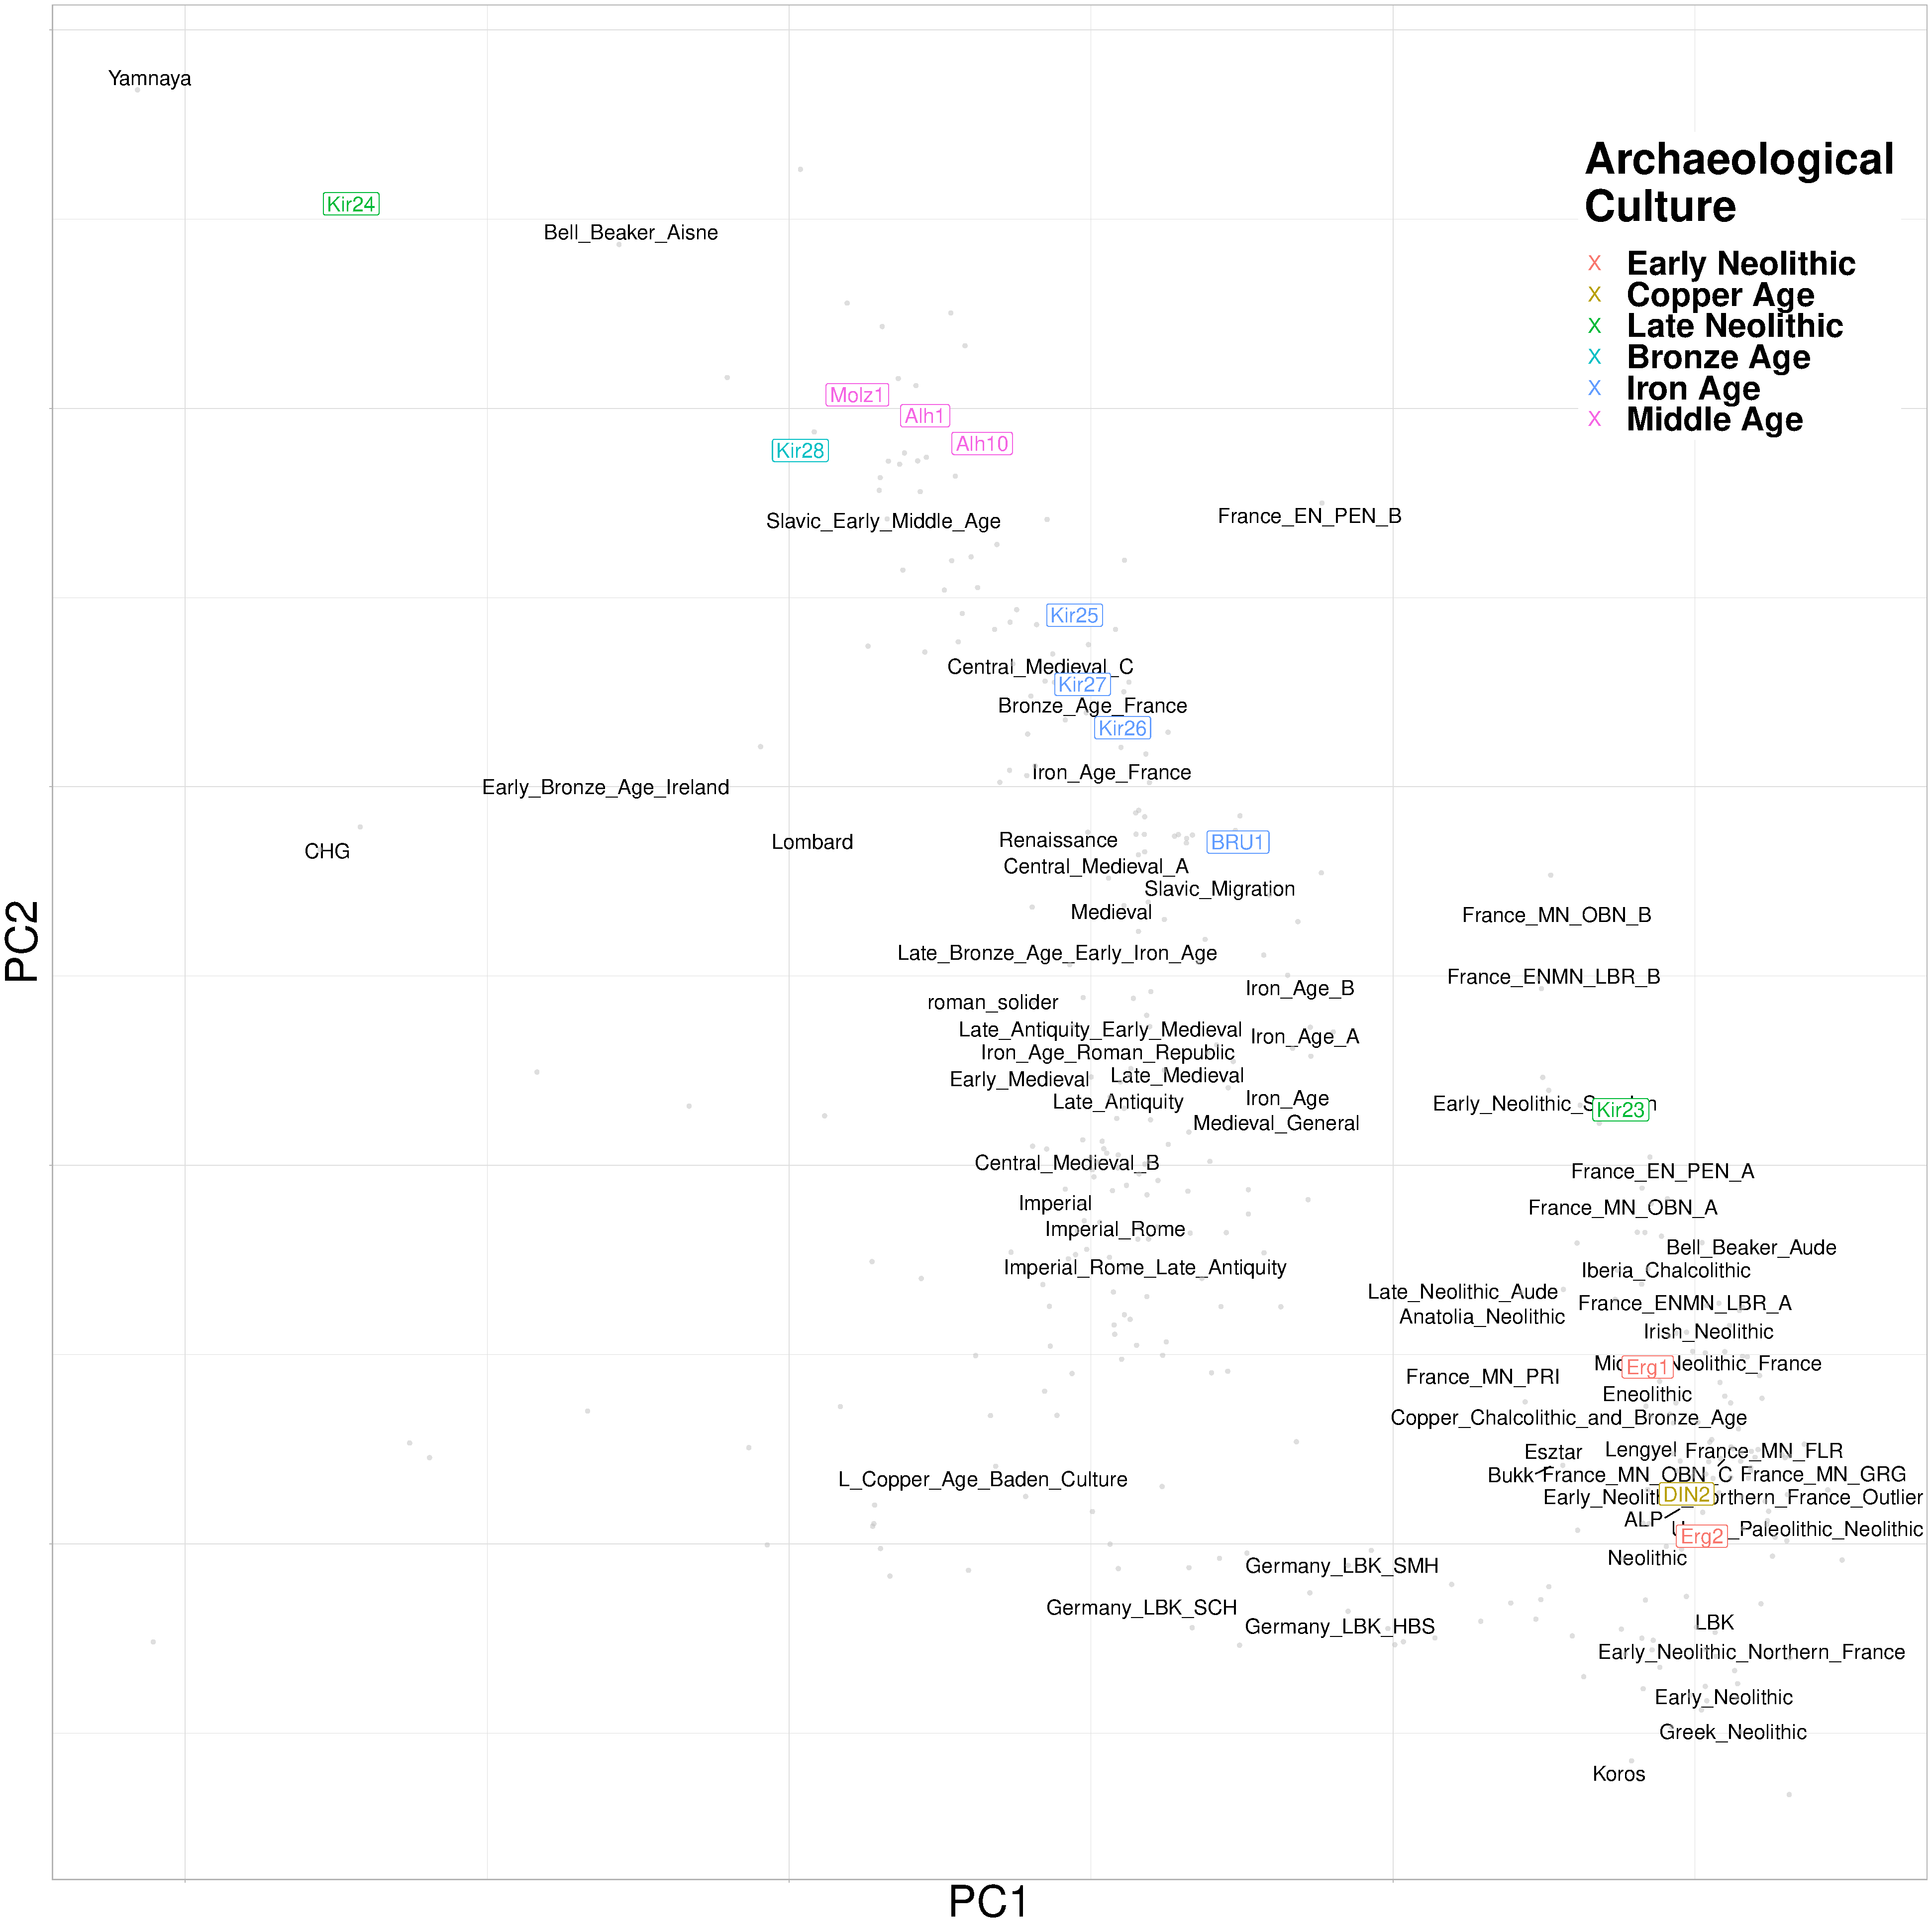
\includegraphics[width=1.0\textwidth]{../images/appendix/plink_withHG_PCA.pdf}
    \caption{Principle component analysis of genotype matrix using plink2. Grey points indicate principle component coordiantes for each sample. Black text indicated mean principle component coordinates for all individuals within that group. Coloured labels represent newly sequenced ancient samples. }
    \label{fig:plink_PCA_HG}
\end{figure}

\begin{figure}[htp]
    \centering
    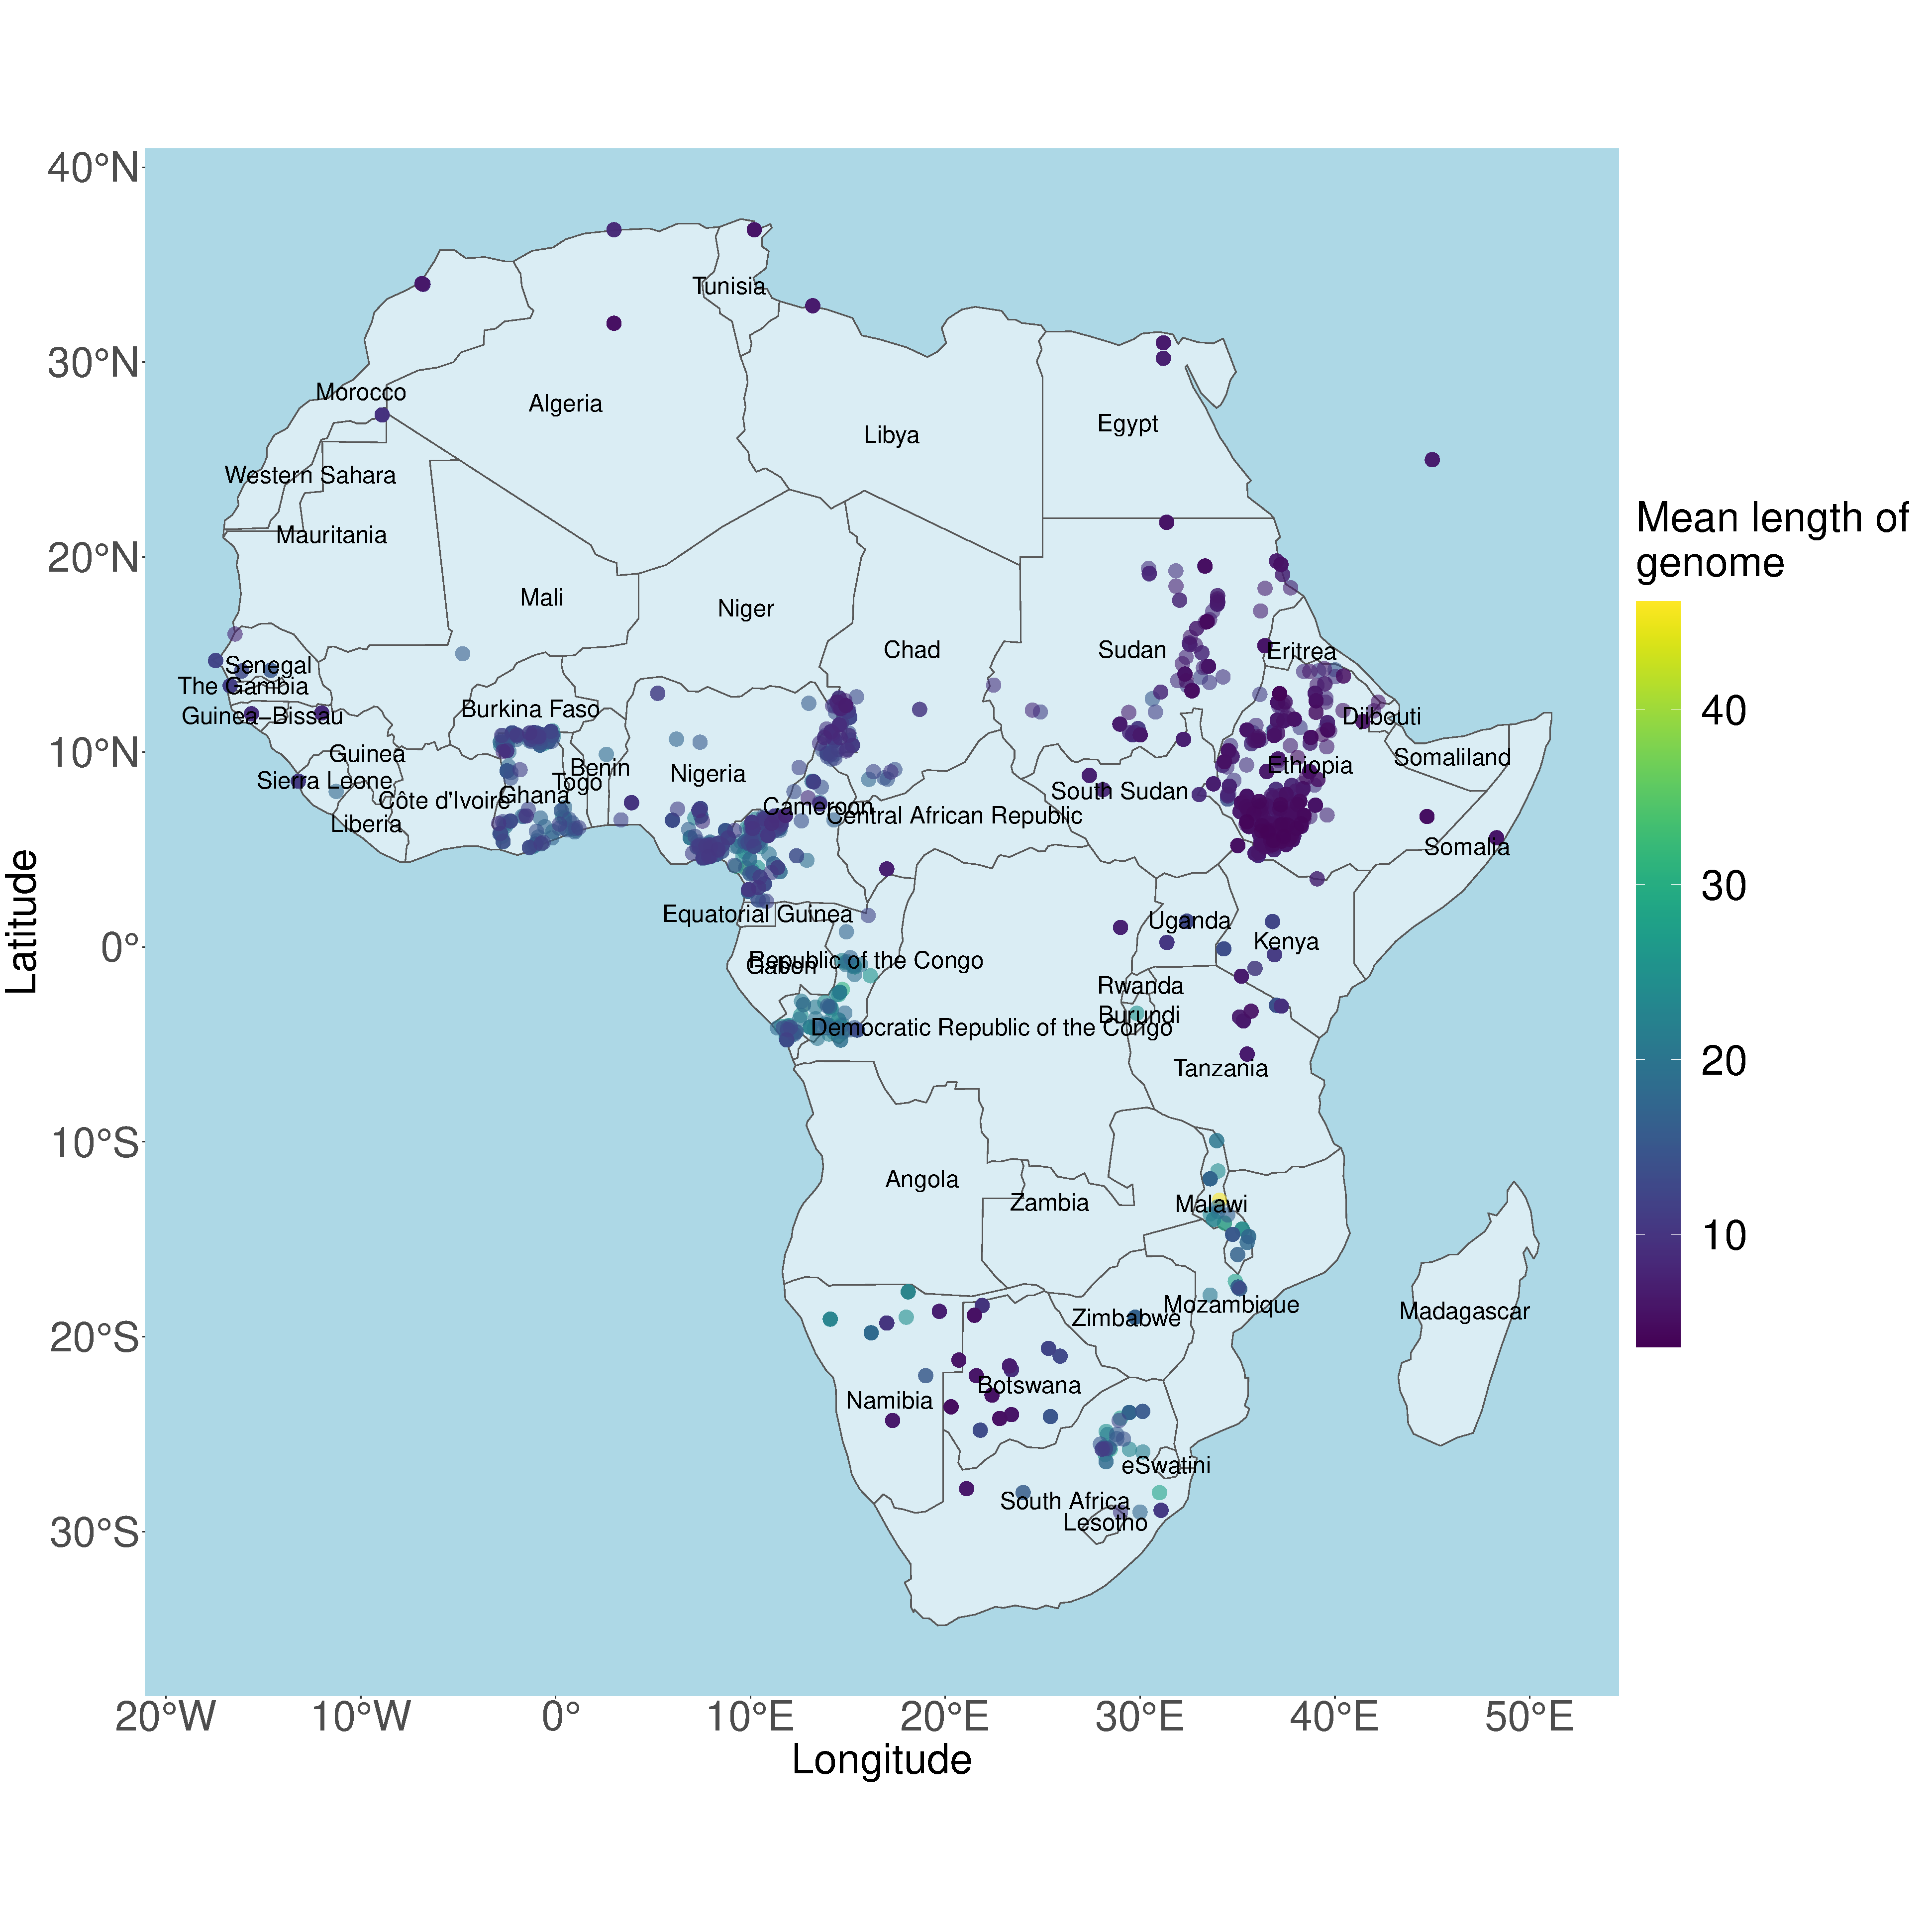
\includegraphics[width=1.0\textwidth]{../images/appendix/haplotype_map_Brazil.pdf}
    \caption{Principle component analysis of genotype matrix using plink2. Grey points indicate principle component coordiantes for each sample. Black text indicated mean principle component coordinates for all individuals within that group. Coloured labels represent newly sequenced ancient samples. }
    \label{fig:haplotype_map_Brazil}
\end{figure}

\begin{figure}[htp]
    \centering
    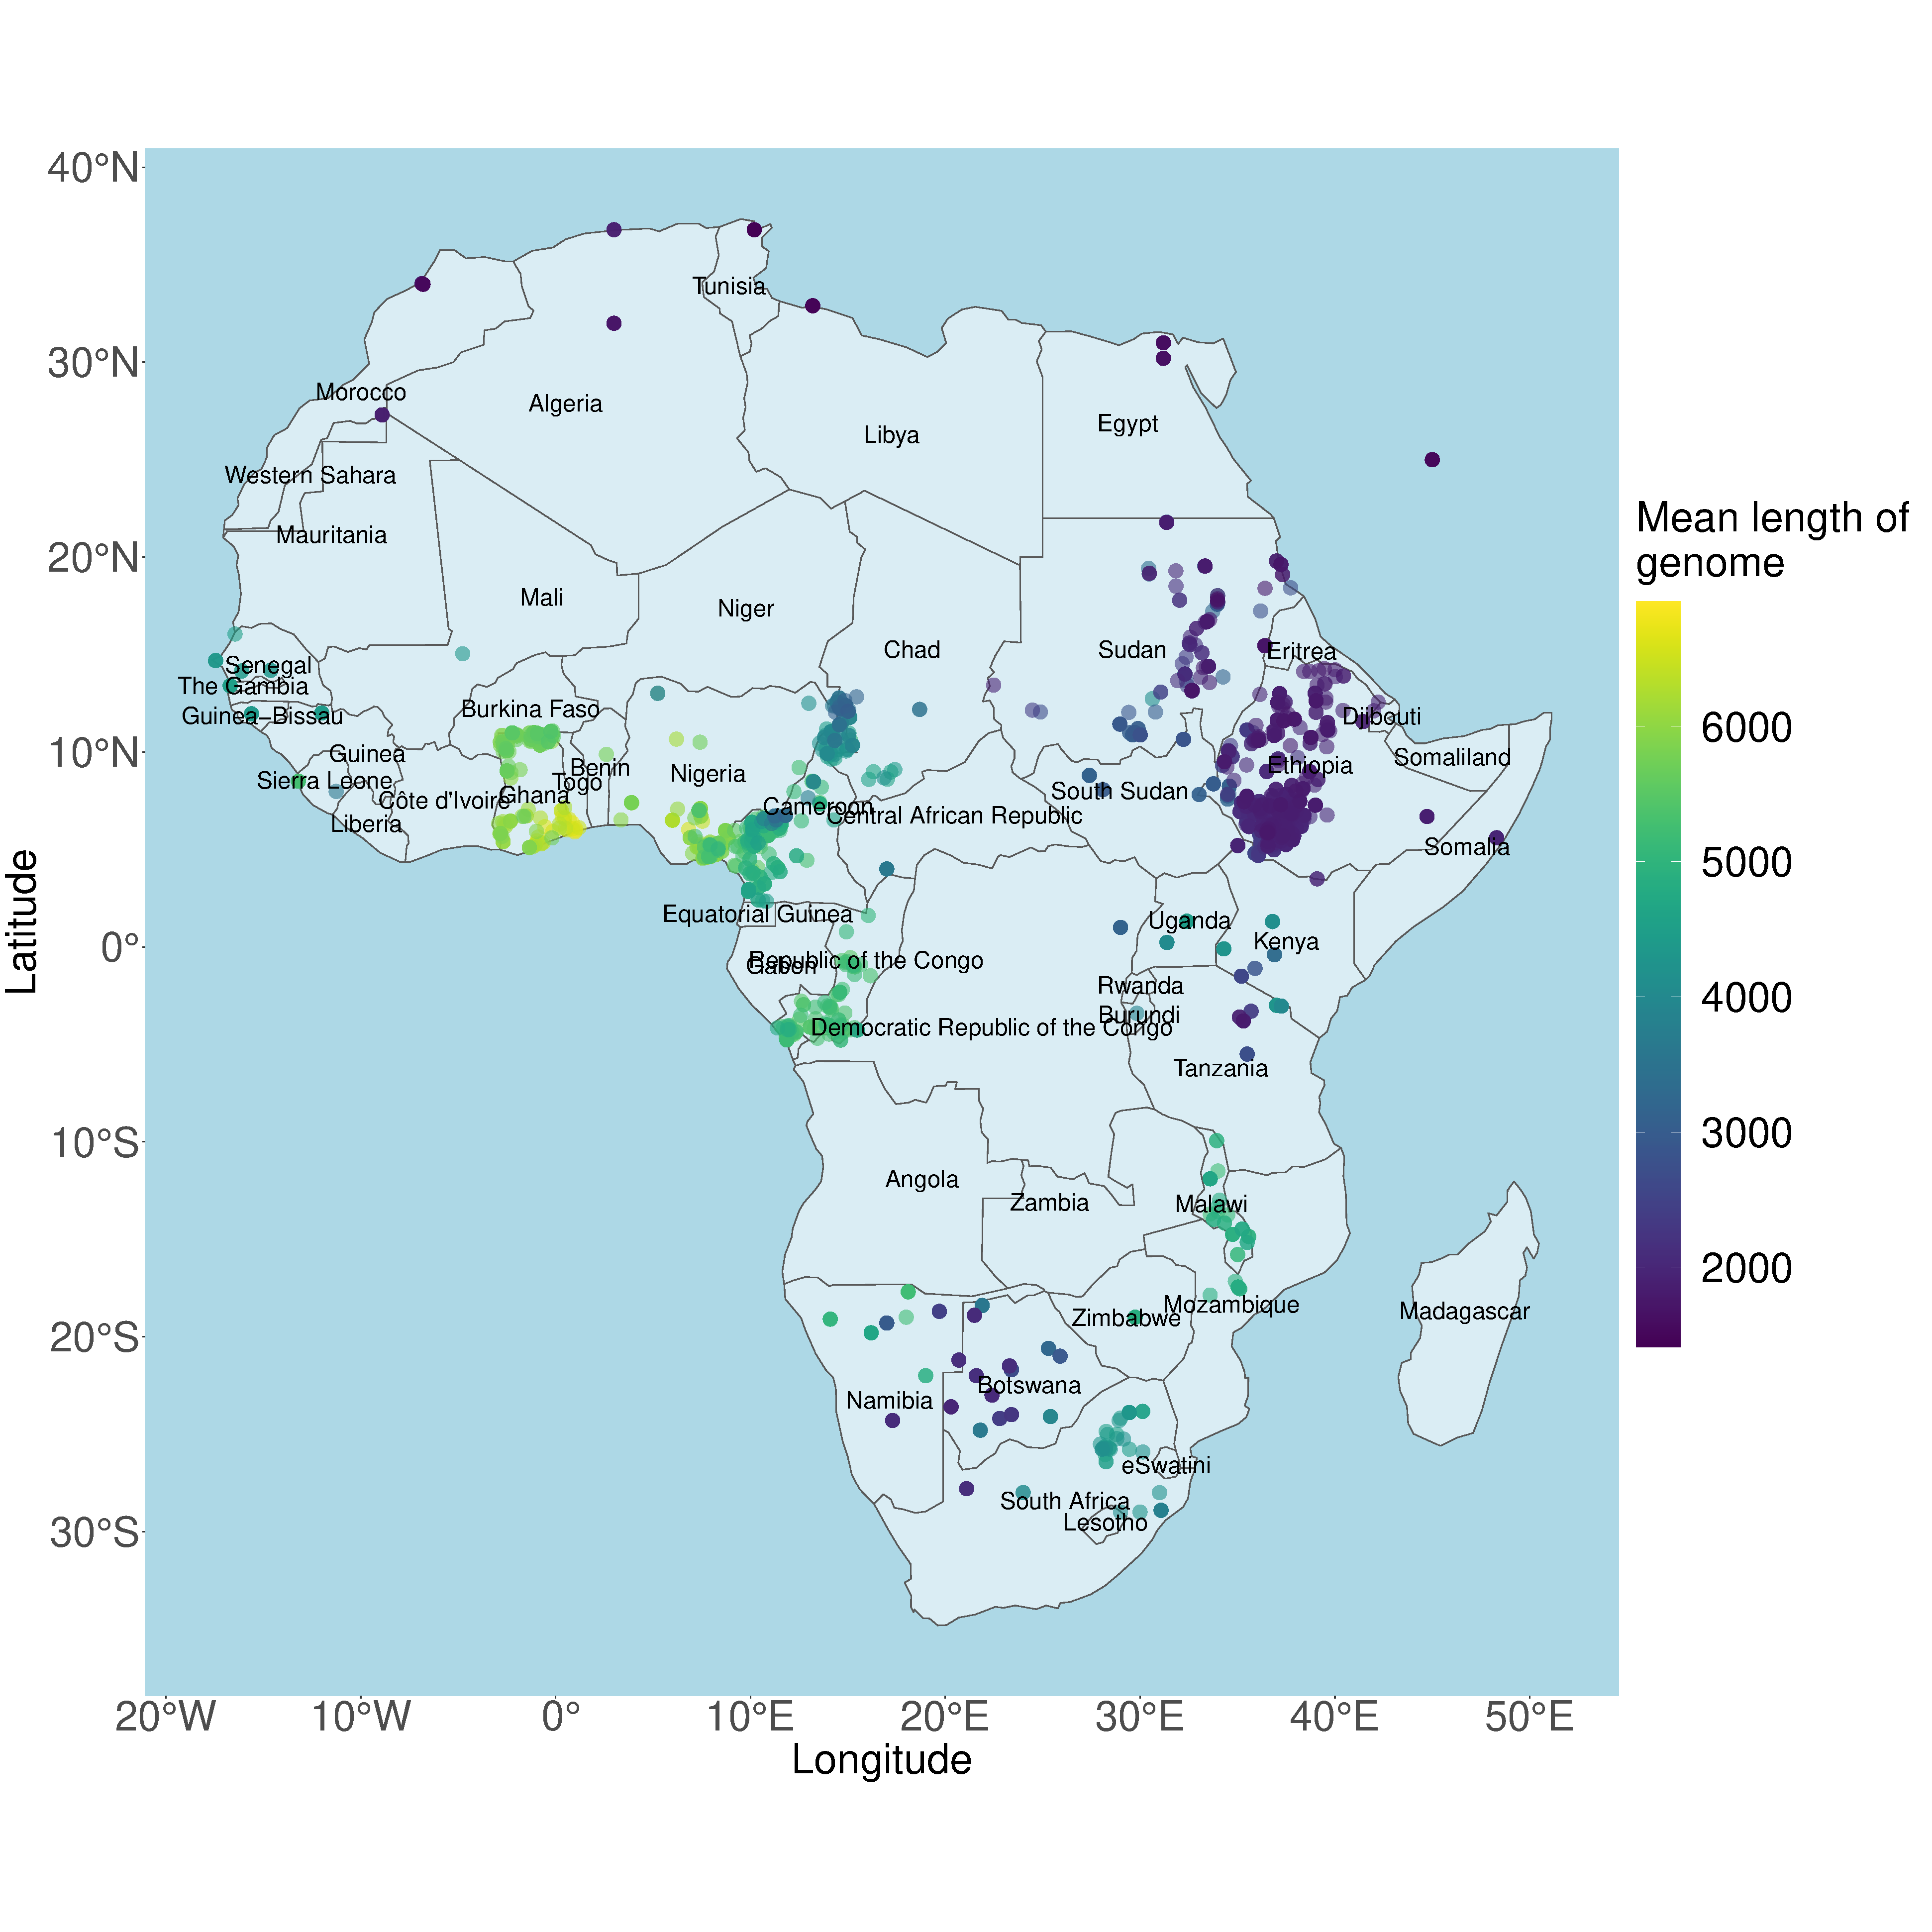
\includegraphics[width=1.0\textwidth]{../images/appendix/haplotype_map_Caribbean.pdf}
    \caption{Principle component analysis of genotype matrix using plink2. Grey points indicate principle component coordiantes for each sample. Black text indicated mean principle component coordinates for all individuals within that group. Coloured labels represent newly sequenced ancient samples.}
    \label{fig:haplotype_map_Caribbean}
\end{figure}


